\documentclass[a4paper,twosided,notoc]{tufte-book}
\usepackage{siunitx}
\hypersetup{colorlinks}% uncomment this line if you prefer colored hyperlinks (e.g., for onscreen viewing)

%%
% Book metadata
\title{tikz-network\\manual}
\author[J\"urgen Hackl]{J\"urgen Hackl}
\publisher{Version 0.2}

%%
% If they're installed, use Bergamo and Chantilly from www.fontsite.com.
% They're clones of Bembo and Gill Sans, respectively.
%\IfFileExists{bergamo.sty}{\usepackage[osf]{bergamo}}{}% Bembo
%\IfFileExists{chantill.sty}{\usepackage{chantill}}{}% Gill Sans

%\usepackage{microtype}

\usepackage{framed}
\definecolor{shadecolor}{HTML}{abd7e6}%{cmyk}{0.49,0.22,.15,0}
\definecolor{hlcolor}{HTML}{057498}%{cmyk}{0.49,0.22,.15,0}
\FrameSep0pt

\usepackage{tikz}
\usetikzlibrary{backgrounds}
\tikzset{background rectangle/.style={fill=yellow!30}}


%%
% Just some sample text
\usepackage{lipsum}

%%
% For nicely typeset tabular material
\usepackage{booktabs}
\usepackage{tabularx}

%%
% For graphics / images
\usepackage{graphicx}
\setkeys{Gin}{width=\linewidth,totalheight=\textheight,keepaspectratio}
\graphicspath{{graphics/}}

% The fancyvrb package lets us customize the formatting of verbatim
% environments.  We use a slightly smaller font.
\usepackage{fancyvrb}
\fvset{fontsize=\normalsize}

%%
% Prints argument within hanging parentheses (i.e., parentheses that take
% up no horizontal space).  Useful in tabular environments.
\newcommand{\hangp}[1]{\makebox[0pt][r]{(}#1\makebox[0pt][l]{)}}

%%
% Prints an asterisk that takes up no horizontal space.
% Useful in tabular environments.
\newcommand{\hangstar}{\makebox[0pt][l]{*}}

%%
% Prints a trailing space in a smart way.
\usepackage{xspace}

%%
% Some shortcuts for Tufte's book titles.  The lowercase commands will
% produce the initials of the book title in italics.  The all-caps commands
% will print out the full title of the book in italics.
\newcommand{\vdqi}{\textit{VDQI}\xspace}
\newcommand{\ei}{\textit{EI}\xspace}
\newcommand{\ve}{\textit{VE}\xspace}
\newcommand{\be}{\textit{BE}\xspace}
\newcommand{\VDQI}{\textit{The Visual Display of Quantitative Information}\xspace}
\newcommand{\EI}{\textit{Envisioning Information}\xspace}
\newcommand{\VE}{\textit{Visual Explanations}\xspace}
\newcommand{\BE}{\textit{Beautiful Evidence}\xspace}

\newcommand{\TL}{Tufte-\LaTeX\xspace}

% Prints the month name (e.g., January) and the year (e.g., 2008)
\newcommand{\monthyear}{%
  \ifcase\month\or January\or February\or March\or April\or May\or June\or
  July\or August\or September\or October\or November\or
  December\fi\space\number\year
}


% Prints an epigraph and speaker in sans serif, all-caps type.
\newcommand{\openepigraph}[2]{%
  %\sffamily\fontsize{14}{16}\selectfont
  \begin{fullwidth}
  \sffamily\large
  \begin{doublespace}
  \noindent\allcaps{#1}\\% epigraph
  \noindent\allcaps{#2}% author
  \end{doublespace}
  \end{fullwidth}
}

% Inserts a blank page
\newcommand{\blankpage}{\newpage\hbox{}\thispagestyle{empty}\newpage}

\usepackage{units}

% Typesets the font size, leading, and measure in the form of 10/12x26 pc.
\newcommand{\measure}[3]{#1/#2$\times$\unit[#3]{pc}}

% Macros for typesetting the documentation
\newcommand{\hlred}[1]{\textcolor{hlcolor}{#1}}% prints in red
\newcommand{\hangleft}[1]{\makebox[0pt][r]{#1}}
\newcommand{\hairsp}{\hspace{1pt}}% hair space
\newcommand{\hquad}{\hskip0.5em\relax}% half quad space
\newcommand{\TODO}{\textcolor{red}{\bf TODO!}\xspace}
\newcommand{\na}{\quad--}% used in tables for N/A cells
\providecommand{\XeLaTeX}{X\lower.5ex\hbox{\kern-0.15em\reflectbox{E}}\kern-0.1em\LaTeX}
\newcommand{\tXeLaTeX}{\XeLaTeX\index{XeLaTeX@\protect\XeLaTeX}}
% \index{\texttt{\textbackslash xyz}@\hangleft{\texttt{\textbackslash}}\texttt{xyz}}
\newcommand{\tuftebs}{\symbol{'134}}% a backslash in tt type in OT1/T1
\newcommand{\doccmdnoindex}[2][]{\texttt{\tuftebs#2}}% command name -- adds backslash automatically (and doesn't add cmd to the index)
\newcommand{\doccmddef}[2][]{%
  \hlred{\texttt{\tuftebs#2}}\label{cmd:#2}%
  \ifthenelse{\isempty{#1}}%
    {% add the command to the index
      \index{#2 command@\protect\hangleft{\texttt{\tuftebs}}\texttt{#2}}% command name
    }%
    {% add the command and package to the index
      \index{#2 command@\protect\hangleft{\texttt{\tuftebs}}\texttt{#2} (\texttt{#1} package)}% command name
      \index{#1 package@\texttt{#1} package}\index{packages!#1@\texttt{#1}}% package name
    }%
}% command name -- adds backslash automatically
\newcommand{\doccmd}[2][]{%
  \texttt{\tuftebs#2}%
  \ifthenelse{\isempty{#1}}%
    {% add the command to the index
      \index{#2 command@\protect\hangleft{\texttt{\tuftebs}}\texttt{#2}}% command name
    }%
    {% add the command and package to the index
      \index{#2 command@\protect\hangleft{\texttt{\tuftebs}}\texttt{#2} (\texttt{#1} package)}% command name
      \index{#1 package@\texttt{#1} package}\index{packages!#1@\texttt{#1}}% package name
    }%
}% command name -- adds backslash automatically
\newcommand{\docopt}[1]{\ensuremath{\langle}\textrm{\textit{#1}}\ensuremath{\rangle}}% optional command argument
\newcommand{\docarg}[1]{\textrm{\textit{#1}}}% (required) command argument
%%%\newenvironment{docspec}{\begin{shaded}\begin{quotation}\ttfamily\parskip0pt\parindent0pt\ignorespaces}{\end{quotation}\end{shaded}}% command specification environment
\newenvironment{docspecdef}{\begin{quotation}\ttfamily\parskip0pt\parindent0pt\ignorespaces}{\end{quotation}}% command specification environment
\newcommand{\docenv}[1]{\texttt{#1}\index{#1 environment@\texttt{#1} environment}\index{environments!#1@\texttt{#1}}}% environment name
\newcommand{\docenvdef}[1]{\hlred{\texttt{#1}}\label{env:#1}\index{#1 environment@\texttt{#1} environment}\index{environments!#1@\texttt{#1}}}% environment name
\newcommand{\docpkg}[1]{\texttt{#1}\index{#1 package@\texttt{#1} package}\index{packages!#1@\texttt{#1}}}% package name
\newcommand{\doccls}[1]{\texttt{#1}}% document class name
\newcommand{\docclsopt}[1]{\texttt{#1}\index{#1 class option@\texttt{#1} class option}\index{class options!#1@\texttt{#1}}}% document class option name
\newcommand{\docclsoptdef}[1]{\hlred{\texttt{#1}}\label{clsopt:#1}\index{#1 class option@\texttt{#1} class option}\index{class options!#1@\texttt{#1}}}% document class option name defined
\newcommand{\docmsg}[2]{\bigskip\begin{fullwidth}\noindent\ttfamily#1\end{fullwidth}\medskip\par\noindent#2}
\newcommand{\docfilehook}[2]{\texttt{#1}\index{file hooks!#2}\index{#1@\texttt{#1}}}
\newcommand{\doccounter}[1]{\texttt{#1}\index{#1 counter@\texttt{#1} counter}}


\newenvironment{docspec}{\begin{shaded}}{\vspace{-5mm}\end{shaded}}% command specification environment


% Numerate the sections
\setcounter{secnumdepth}{2}

\setcounter{tocdepth}{3}


\usepackage{etoolbox}

\makeatletter
\patchcmd{\ttlh@hang}{\parindent\z@}{\parindent\z@\leavevmode}{}{}
%\patchcmd{\ttlh@hang}{\noindent}{}{}{}
\patchcmd{\ttlh@hang}{\noindent}{}{}{}
\makeatother


% chapter format
\titleformat{\chapter}%
  {\huge\rmfamily\itshape}% format applied to label+text
  {\llap{\parbox{1.5cm}{\hfill\itshape\huge\thechapter}\hspace{2mm}}}% label
  {0em}% horizontal separation between label and title body
  {}% before the title body
  []% after the title body

% section format
\titleformat{\section}%
  {\normalfont\Large\itshape}% format applied to label+text
  {\llap{\parbox{1.0cm}{\hfill\thesection}\hspace{2mm}}}% label
  {0em}% horizontal separation between label and title body
  {}% before the title body
  []% after the title body

% subsection format
\titleformat{\subsection}%
  {\normalfont\large\itshape}% format applied to label+text
  {\llap{\parbox{1.5cm}{\hfill\thesubsection}\hspace{2mm}}}% label
  {0em}% horizontal separation between label and title body
  {}% before the title body
  []% after the title body

\newcommand{\pkg}{\doccls{tikz-network}\xspace}
\newcommand{\tikzsym}{Ti\emph{k}Z }

\usepackage{listings}
\lstset{ %
basicstyle=\small\linespread{.8}\ttfamily,
commentstyle=\itshape\color{black!70},
stepnumber=2,
showspaces=false,
showstringspaces=false,
showtabs=false,
tabsize=2,
captionpos=b,
breaklines=true,
breakatwhitespace=false,
title=\lstname,
escapeinside={+*}{*+},
morekeywords={*,...},
stringstyle=\ttfamily,
emphstyle={\color{red}\bfseries},
}

\usepackage{../tikz-network}


% Generates the index
\usepackage{makeidx}
\makeindex

\renewcommand{\chaptermark}[1]{%
\markboth{#1}{}}

\fancyhead[LE]{\thepage\quad\smallcaps{\newlinetospace{\leftmark}}}

\begin{document}


%\maketitle

\thispagestyle{empty}

  \begin{fullwidth}%
\sffamily%
  \fontsize{18}{20}\selectfont\par\noindent\textcolor{darkgray}{\allcaps{\thanklessauthor}}%
  \vspace{11.5pc}%
  \fontsize{36}{40}\selectfont\par\noindent\textcolor{darkgray}{\allcaps{\thanklesstitle}}%
\vspace{3cm}
\begin{center}
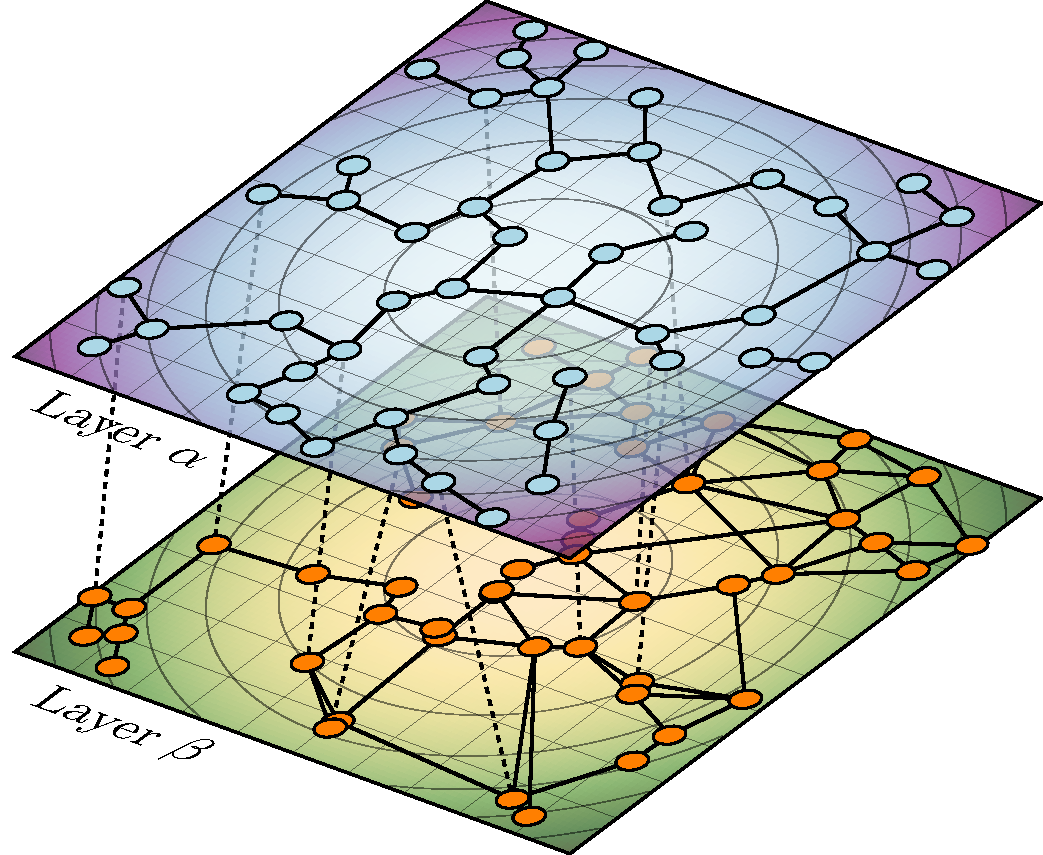
\includegraphics[width=14cm]{graphics/front.pdf}%
\end{center}
\vfill%
  \fontsize{14}{16}\selectfont\par\noindent\allcaps{\thanklesspublisher}%
  \end{fullwidth}%


\newpage

\begin{fullwidth}
\begin{tikzpicture}[remember picture, overlay]
 \node[rectangle,inner sep=2pt,fill=red!30,draw=black,text width=12cm] at ($(current page.center)+(0,6)$) {%
  The \pkg package is still under development. Hence, changes in the commands and functionality cannot be excluded. 
};
\end{tikzpicture}

~\vfill
\thispagestyle{empty}
\setlength{\parindent}{0pt}
\setlength{\parskip}{\baselineskip}
Copyright \copyright\ \the\year\ \thanklessauthor

\par\smallcaps{\thanklesspublisher}
\par\smallcaps{\url{https://github.com/hackl/tikz-network}}

\par\textit{Released, \monthyear}
\end{fullwidth}

\begin{fullwidth}
\tableofcontents
\end{fullwidth}

\cleardoublepage
\chapter{Introduction}

In recent years, complex network theory becomes more and more popular within the scientific community. Besides a solid mathematical base on which these theories are built on, a visual representation of the networks allow communicating complex relationships to a broad audience.

Nowadays, a variety of great visualization tools are available, which helps to structure, filter, manipulate and of course to visualize the networks. However, they come with some limitations, including the need for specific software tools, difficulties to embed the outputs properly in a \LaTeX~file (e.g. font type, font size, additional equations and math symbols needed, \dots) and challenges in the post-processing of the graphs, without rerunning the software tools again.

In order to overcome this issues, the package \pkg was created. Some of the features are:

\begin{itemize}
\item \LaTeX~ is a standard for scientific publications and widely used
\item beside \LaTeX~ no other software is needed
\item no programming skills are needed
\item simple to use but allows 100\% control over the output
\item easy for post-processing (e.g. adding drawings, texts, equations,\dots)
\item same fonts, font sizes, mathematical symbols, \dots as in the document
\item no quality loss of the output due to the pdf format
\item networks are easy to adapt or modify for lectures or small examples
\item able to visualize larger networks
\item three-dimensional visualization of (multilayer) networks
\item compatible with other visualization tools
\end{itemize}
\newpage

\section{How to read this manual?}

The aim of this manual is to describe the use of the \pkg library for visualizing networks. To ensure an easy use of the elements and to keep the clarity, this manual is structured as follows:
\begin{itemize}
\item In Chapter \ref{chap:simple_networks} the elements to create simple networks (by hand) in a plane are explained. Thereby, the use of the commands \doccmd{Vertex} and \doccmd{Edge} are shown.
\item How to create complex networks from external files\footnote{e.g. \doccls{igraph} or \doccls{networkx}} are explained in Chapter \ref{chap:complex_networks}. The main commands, therefore are \doccmd{Vertices} and \doccmd{Edges} which are using the same options as in the simple case.
\item In Chapter \ref{chap:multilayer_networks}, the visualization of multilayer networks is explained. Additional visualization tools such as \doccmd{Plain} and \docenv{Layer} are introduced.
\item The default settings used and how they can be modified is explained in Chapter \ref{chap:default_settings}.
\item Information about troubleshooting and support is given in Chapter \ref{chap:troubleshooting}
\item Since this is the alpha version (0.1) of the package, features which will be probably added and commands which have to be fixed are listed in Appendix \ref{chap:todo}.
\end{itemize}

\subsection{A few explanations}

The images in this manual are created with the \pkg library or \tikzsym. The code used for this is
specified for each image.
\begin{marginfigure}[30mm]
\centering
  \begin{tikzpicture}%[framed]
    \filldraw (-.2,.2) circle (2pt) (.2,.2) circle (2pt);
    \draw (0,0) circle (5mm) (-.3,-.1) .. controls (0,-.3) .. (.3,-.1);
  \end{tikzpicture}
\end{marginfigure}

\begin{docspec}
\begin{lstlisting}
  \begin{tikzpicture}
    \filldraw (-.2,.2) circle (2pt) (.2,.2) circle (2pt);
    \draw (0,0) circle (5mm) (-.3,-.1) .. controls (0,-.3) .. (.3,-.1);
  \end{tikzpicture}
\end{lstlisting}
\end{docspec}

Special additions which are needed for a better understanding are shown in orange but are not in the sample code available.

\begin{marginfigure}[23mm]
\centering
  \begin{tikzpicture}%[framed]
    \filldraw [orange] (0,0) circle (2pt)
    (1,1) circle (2pt)
    (2,1) circle (2pt)
    (2,0) circle (2pt);
    \draw (0,0) .. controls (1,1) and (2,1) .. (2,0);
  \end{tikzpicture}
\end{marginfigure}

\begin{docspec}
\begin{lstlisting}
  \begin{tikzpicture}
    \draw (0,0) .. controls (1,1) and (2,1) .. (2,0);
  \end{tikzpicture}
\end{lstlisting}
\end{docspec}

\subsection{Inputs}
\label{sec:inputs}

The commands in the \pkg library (e.g. \doccmd{Vertex}, \doccmd{Edge}) always start with capital letters and DO NOT need a semicolon <<;>> at the end. Boolean arguments start also with capital letters (e.g. \docopt{NoLabel}). Arguments which need an user input, use are written in small letters (e.g. \docopt{color}).

Basically, one can distinguish between the mandatory argument $\{~\}$ and the optional argument $[~]$. The first values must be entered compulsory. By contrast, nothing has to be entered for the optional input. Additional features (e.g. \docopt{size})) can be activated when entering optional parameters.

When entering size values the base unit is always predefined in $[cm]$\footnote{The default unit can be changed with \doccmd{SetDefaultUnit}; see Section~\ref{sec:gerneral_settings}}, except for line widths which are dedined in $[pt]$. Percentage values $\%$ are always specified as decimal values; for example, $100\% = 1.0 $ and $ 10 \% $ corresponds to $ 0.1 $.


\subsection{Additional help}

Is the manual not enough, occur some ambiguities or some \tikzsym commands are unclear, please have a look in the ``\tikzsym and PGF Manual'' from Till Tantau\footnote{\url{http://mirror.switch.ch/ftp/mirror/tex/graphics/pgf/base/doc/pgfmanual.pdf}}.

Should you have any further questions, please do not hesitate to contact me. 

\section{Installation}
\label{sec:Installation}

Actually, we can hardly speak of an installation since only the necessary package \pkg must be loaded in the preamble of your document.

The current release of the package is available via CTAN\footnote{\TODO upload the package to CTAN, and add here the link}. A release candidate for the next version of \pkg is available on github\footnote{\url{https://github.com/hackl/}}

Is the package installed or the style file is stored in the folder of the main file, so the library can be imported, as the following example shows:

\begin{docspec}
\begin{lstlisting}
  % ------------
  % header
  \documentclass{scrreprt}

  % ------------
  % packages
  \usepackage{tikz-network}
\end{lstlisting}
\end{docspec}

\section{Additional necessary packages}

To use all commands and options of \tikzsym, possibly some packages need to be reloaded. These missing files (or their names) appear in the error log when you convert the file. However, for the package described in this manual, it is sufficient to use the library and the \tikzsym standard commands.

\chapter{Simple Networks}
\label{chap:simple_networks}

\section{Vertex}
\label{sec:vertex}
On essential command is \doccmddef{Vertex}, which allow placing vertices in the document and modify their appearance. 
\begin{docspecdef}
  \doccmd{Vertex}[\docopt{local options}]\{\docarg{Name}\}
\end{docspecdef}
In order to be able to place a vertex, a non-empty \docarg{Name} argument is required. This argument defines the vertex's reference name, which must be unique. Mathematical symbols are not allowed as name as well as no blank spaces. The \docarg{Name} should not be confused with the \docopt{label}, that is used for display; for example one may want to display $A_1$ while the name will be \docarg{A1}. 

For a \doccmd{Vertex} the following options are available:

\begin{table}[h]\index{Vertex!options}
  \footnotesize%
  \begin{center}
    \begin{tabular}{lccl}
      \toprule
      Option & Default & Type &Definition \\
      \midrule
      x          & 0     & measure& x-coordinate \\
      y          & 0     & measure& y-coordinate \\
      size       & \{\}  & measure& diameter of the circle\\
      color      & \{\}  & color & fillcolor of vertex\\
      opacity    & \{\}  & number & opacity of the fill color \\
      label      & \{\}  & string & label \\
      position   & center& value$^a$ & label position\\
      distance   & 0     & measure & label distance from the center \\
      style      & \{\}  & string & additional \tikzsym styles \\
      layer      & \{\}  & number & assigned layer of the vertex \\
      \midrule
      NoLabel    & false & boolean & delete the label \\
      IdAsLabel  & false & boolean & uses the \docarg{Name} as label \\
      Math       & false & boolean & displays the label in math mode \\
      RGB        & false & boolean & allow RGB colors \\
      \bottomrule
    \end{tabular}
    \scriptsize
    \\$^a$ either measure or string
  \end{center}
  \caption{Local options for the \doccmd{Vertex} command.}
  \label{tab:vertex_options}
\end{table}

The order how the options are entered does not matter. Changes to the default Vertex layout can be made with \doccmd{SetVertexStyle}\footnote{see Section \ref{sec:vertex_style}}

\begin{docspecdef}
  \doccmd{Vertex}[\docopt{x}=\docarg{measure},\docopt{y}=\docarg{measure}]\{\docarg{Name}\}
\end{docspecdef}

The location of the vertices are determined by Cartesian coordinates in \docopt{x} and \docopt{y}. The coordinates are optional. If no coordinates are determined the vertex will be placed at the origin ($0,0$). The entered \docarg{measure} are in default units (\si{cm}). Changing the unites (locally) can be done by adding the unit to the \docarg{measure}\footnote{e.g. x=\SI{1}{in}}. Changes to the default setting can be made with \doccmd{SetDefaultUnit}\footnote{see Section \ref{sec:gerneral_settings}}. 
\newpage
\begin{marginfigure}[6mm]
\centering
  \begin{tikzpicture}
    \Vertex{A}
    \Vertex[x=1,y=1]{B}
    \Vertex[x=2]{C}
    \node at (0,0)[font=\footnotesize,orange]{\textbf{A}};
    \node at (1,1)[font=\footnotesize,orange]{\textbf{B}};
    \node at (2,0)[font=\footnotesize,orange]{\textbf{C}};
  \end{tikzpicture}
\end{marginfigure}

\begin{docspec}
\begin{lstlisting}
  \begin{tikzpicture}
    \Vertex{A}
    \Vertex[x=1,y=1]{B}
    \Vertex[x=2]{C}
  \end{tikzpicture}
\end{lstlisting}
\end{docspec}

\begin{docspecdef}
  \doccmd{Vertex}[\docopt{size}=\docarg{measure}]\{\docarg{Name}\}
\end{docspecdef}

The diameter of the vertex can be changed with the option \docopt{size}. Per default a vertex has \SI{0.6}{cm} in diameter. Also, here the default units are \si{cm} and have not to be added to the \docarg{measure}.

\begin{marginfigure}[34mm]
\centering
  \begin{tikzpicture}
    \Vertex[size=.3]{A}
    \Vertex[x=1,size=.7]{B}
    \Vertex[x=2.3,size=1]{C}
  \end{tikzpicture}
\end{marginfigure}

\begin{docspec}
\begin{lstlisting}
  \begin{tikzpicture}
    \Vertex[size=.3]{A}
    \Vertex[x=1,size=.7]{B}
    \Vertex[x=2.3,size=1]{C}
  \end{tikzpicture}
\end{lstlisting}
\end{docspec}

\begin{docspecdef}
  \doccmd{Vertex}[\docopt{color}=\docarg{color}]\{\docarg{Name}\}
\end{docspecdef}

To change the fill color of each vertex individually, the option \docopt{color} has to be used. Without the option \docopt{RGB} set, the default \tikzsym and \LaTeX~ colors can be applied. 

\begin{marginfigure}[34mm]
\centering
  \begin{tikzpicture}
    \Vertex[color = blue]{A}
    \Vertex[x=1,color=red]{B}
    \Vertex[x=2,color=green!70!blue]{C}
  \end{tikzpicture}
\end{marginfigure}

\begin{docspec}
\begin{lstlisting}
  \begin{tikzpicture}
    \Vertex[color = blue]{A}
    \Vertex[x=1,color=red]{B}
    \Vertex[x=2,color=green!70!blue]{C}
  \end{tikzpicture}
\end{lstlisting}
\end{docspec}


\begin{docspecdef}
  \doccmd{Vertex}[\docopt{opacity}=\docarg{number}]\{\docarg{Name}\}
\end{docspecdef}

With the option \docopt{opacity} the opacity of the vertex fill color can be modified. The range of the \docarg{number} lies between $0$ and $1$. Where $0$ represents a fully transparent fill and $1$ a solid fill.

\begin{marginfigure}[34mm]
\centering
  \begin{tikzpicture}
    \draw[thick,orange,dashed] (-.5,0) -- (2.5,0);
    \Vertex[opacity = 1]{A}
    \Vertex[x=1,opacity =.7]{B}
    \Vertex[x=2,opacity =.2]{C}
  \end{tikzpicture}
\end{marginfigure}

\begin{docspec}
\begin{lstlisting}
  \begin{tikzpicture}
    \Vertex[opacity = 1]{A}
    \Vertex[x=1,opacity =.7]{B}
    \Vertex[x=2,opacity =.2]{C}
  \end{tikzpicture}
\end{lstlisting}
\end{docspec}

\begin{docspecdef}
  \doccmd{Vertex}[\docopt{label}=\docarg{string}]\{\docarg{Name}\}
\end{docspecdef}

In \pkg there are several ways to define the labels of the vertices and edges. The common way is via the option \docopt{label}. Here, any \docarg{string} argument can be used, including blank spaces. The environment \$ \$ can be used to display mathematical expressions. 

\begin{marginfigure}[34mm]
\centering
  \begin{tikzpicture}
    \Vertex[label=foo]{A}
    \Vertex[x=1,label=bar]{B}
    \Vertex[x=2,label=$u_1$]{B}
  \end{tikzpicture}
\end{marginfigure}

\begin{docspec}
\begin{lstlisting}
  \begin{tikzpicture}
    \Vertex[label=foo]{A}
    \Vertex[x=1,label=bar]{B}
    \Vertex[x=2,label=$u_1$]{B}
  \end{tikzpicture}
\end{lstlisting}
\end{docspec}


\begin{docspecdef}
  \doccmd{Vertex}[\docopt{label}=\docarg{string},\docopt{position}=\docarg{value},\docopt{distance}=\docarg{number}]\{\docarg{Name}\}
\end{docspecdef}

Per default the \docopt{position} of the \docopt{label} is in the \docarg{center} of the vertex. Classical \tikzsym commands\footnote{e.g. \docarg{above}, \docarg{below}, \docarg{left}, \docarg{right}, \docarg{above left}, \docarg{above right},\dots} can be used to change the \docopt{position} of the \docopt{label}. Instead, using such command, the position can be determined via an angle, by entering a \docarg{number} between $-360$ and $360$. The origin ($0^\circ$) is the $y$ axis. A positive \docarg{number} change the \docopt{position} counter clockwise, while a negative \docarg{number} make changes clockwise.

With the option, \docopt{distance} the distance between the vertex and the label can be changed. 

\begin{marginfigure}[31mm]
\centering
  \begin{tikzpicture}
    \Vertex[label=A,position=below]{A}
    \Vertex[x=1,label=B,position=below,distance=2mm]{B}
    \Vertex[x=2,label=C,position=30,distance=1mm]{C}
    \draw[orange,dashed](2,0) --++ (7mm,0mm)(2,0)--++(30:7mm);
    \draw[orange,->] (2.5,0) arc (0:30:5mm);
    \node[orange] (x) at (2.6,-.2) {$30^\circ$};
  \end{tikzpicture}
\end{marginfigure}

\begin{docspec}
\begin{lstlisting}
  \begin{tikzpicture}
    \Vertex[label=A,position=below]{A}
    \Vertex[x=1,label=B,position=below,distance=2mm]{B}
    \Vertex[x=2,label=C,position=30,distance=1mm]{C}
  \end{tikzpicture}
\end{lstlisting}
\end{docspec}

\begin{docspecdef}
  \doccmd{Vertex}[\docopt{style}=\{\docarg{string}\}]\{\docarg{Name}\}
\end{docspecdef}

Any other \tikzsym style option or command can be entered via the option \docopt{style}. Most of these commands can be found in the ``\tikzsym and PGF Manual''. Contain the commands additional options (e.g.\docopt{shading}=\docarg{ball}), then the argument for the \docopt{style} has to be between $\{~\}$ brackets.

\begin{marginfigure}[32mm]
\centering
  \begin{tikzpicture}
    \Vertex[style={color=green}]{A}
    \Vertex[x=1,style=dashed]{B}
    \Vertex[x=2,style={shading=ball}]{C}
  \end{tikzpicture}
\end{marginfigure}

\begin{docspec}
\begin{lstlisting}
  \begin{tikzpicture}
    \Vertex[style={color=green}]{A}
    \Vertex[x=1,style=dashed]{B}
    \Vertex[x=2,style={shading=ball}]{C}
  \end{tikzpicture}
\end{lstlisting}
\end{docspec}

\begin{docspecdef}
  \doccmd{Vertex}[\docopt{IdAsLabel}]\{\docarg{Name}\}
\end{docspecdef}
\begin{docspecdef}
  \doccmd{Vertex}[\docopt{NoLabel},\docopt{label}=\docarg{string}]\{\docarg{Name}\}
\end{docspecdef}

\docopt{IdAsLabel} is a boolean option which assigns the \docarg{Name} of the vertex as label. On the contrary, \docopt{NoLabel} suppress all labels.

\begin{marginfigure}[32mm]
\centering
  \begin{tikzpicture}
    \Vertex[IdAsLabel]{A}
    \Vertex[x=1,label=B,NoLabel]{B}
    \Vertex[x=2,IdAsLabel,NoLabel]{C}
  \end{tikzpicture}
\end{marginfigure}

\begin{docspec}
\begin{lstlisting}
  \begin{tikzpicture}
    \Vertex[IdAsLabel]{A}
    \Vertex[x=1,label=B,NoLabel]{B}
    \Vertex[x=2,IdAsLabel,NoLabel]{C}
  \end{tikzpicture}
\end{lstlisting}
\end{docspec}

\begin{docspecdef}
  \doccmd{Vertex}[\docopt{Math},\docopt{label}=\docarg{string}]\{\docarg{Name}\}
\end{docspecdef}

The option \docopt{Math} allows transforming labels into mathematical expressions without using the \$~\$ environment. In combination with \docopt{IdAsLabel} allows this option also mathematical expressions by the definition of the vertex \docarg{Name}.

\newpage
\begin{marginfigure}[12mm]
\centering
  \begin{tikzpicture}
    \Vertex[IdAsLabel]{A1}
    \Vertex[x=1,label=B_1,Math]{B}
    \Vertex[x=2,Math,IdAsLabel]{C_1}
  \end{tikzpicture}
\end{marginfigure}

\begin{docspec}
\begin{lstlisting}
  \begin{tikzpicture}
    \Vertex[IdAsLabel]{A1}
    \Vertex[x=1,label=B_1,Math]{B}
    \Vertex[x=2,Math,IdAsLabel]{C_1}
  \end{tikzpicture}
\end{lstlisting}
\end{docspec}


\begin{docspecdef}
  \doccmd{Vertex}[\docopt{RGB},\docopt{color}=\docarg{RGB values}]\{\docarg{Name}\}
\end{docspecdef}

In order to display RGB colors for the vertex fill color, the option \docopt{RGB} has to be entered. In combination with this option, the \docopt{color} hast to be a list with the \docarg{RGB 
values}, separated by <<,>> and within $\{~\}$.\footnote{e.g. the RGB code for white: $\{255,255,255\}$}

\begin{marginfigure}[8mm]
\centering
  \begin{tikzpicture}
    \Vertex[RGB,color={127,201,127}]{A}
    \Vertex[x=1,RGB,color={190,174,212}]{B}
    \Vertex[x=2,RGB,color={253,192,134}]{C}
  \end{tikzpicture}
\end{marginfigure}

\begin{docspec}
\begin{lstlisting}
  \begin{tikzpicture}
    \Vertex[RGB,color={127,201,127}]{A}
    \Vertex[x=1,RGB,color={190,174,212}]{B}
    \Vertex[x=2,RGB,color={253,192,134}]{C}
  \end{tikzpicture}
\end{lstlisting}
\end{docspec}

\begin{docspecdef}
  \doccmd{Vertex}[\docopt{layer}=\docarg{number}]\{\docarg{Name}\}
\end{docspecdef}

With the option \docopt{layer} the vertex can be assigned to a specific layer. More about this option and the use of layers is explained in Chapter~\ref{chap:multilayer_networks}. 

\newpage

\section{Edge}
\label{sec:edge}

The second essential command is an \doccmddef{Edge}, which allow connecting two vertices. 

\begin{docspecdef}
  \doccmd{Edge}[\docopt{local options}](\docarg{Vertex i})(\docarg{Vertex j})
\end{docspecdef}

Edges can be generated between one or two vertices. In the first case, a self-loop will be generated. As mandatory arguments the \docarg{Names} of the vertices which should be connected must be entered between $(~)$ brackets. In case of a directed edge, the order is important. An edge is created from \docarg{Vertex i} (origin) to \docarg{Vertex j} (destination).

For an \doccmd{Edge} the following options are available:

\begin{table}[h]\index{Edge!options}
  \footnotesize%
  \begin{center}
    \begin{tabular}{lccl}
      \toprule
      Option & Default & Type &Definition \\
      \midrule
      lw          & \{\}  & measure & line width of the edge \\
      color       & \{\}  & color   & edge color\\
      opacity     & \{\}  & number  & opacity of the edge \\
      bend        & 0     & number  & angle out/in of the vertex \\
      label       & \{\}  & string  & label \\
      position    & \{\}  & string  & label position\\
      distance    & 0.5   & number  & label distance from Vertex i\\
      style       & \{\}  & string  & additional \tikzsym styles \\
      \midrule
      loopsize    & 1cm   & measure & size parameter of the self-loop\\
      loopposition& 0     & number  & orientation of the self-loop \\
      loopshape   & 90    & number  & loop angle out/in of the vertex \\
      \midrule
      Direct      & false & boolean & allow directed edges \\
      Math        & false & boolean & displays the label in math mode \\
      RGB         & false & boolean & allow RGB colors \\
      \bottomrule
    \end{tabular}
    \scriptsize
  \end{center}
  \caption{Local options for the \doccmd{Edge} command.}
  \label{tab:edge_options}
\end{table}

The options \docopt{loopsize}, \docopt{loopposition}, and \docopt{loopsize} are only for self-loops available.

\begin{docspecdef}
  \doccmd{Edge}(\docarg{Vertex i})(\docarg{Vertex j})
\end{docspecdef}

An edge is created between \docarg{Vertex i} and \docarg{Vertex j}. 

\begin{marginfigure}[28mm]
\centering
  \begin{tikzpicture}
    \Vertex{A} \Vertex[x=2]{B}
    \Edge(A)(B)
  \end{tikzpicture}
\end{marginfigure}

\begin{docspec}
\begin{lstlisting}
  \begin{tikzpicture}
    \Vertex{A} \Vertex[x=2]{B}
    \Edge(A)(B)
  \end{tikzpicture}
\end{lstlisting}
\end{docspec}

\begin{docspecdef}
  \doccmd{Edge}[\docopt{lw}=\docarg{measure}](\docarg{Vertex i})(\docarg{Vertex j})
\end{docspecdef}

The line width of an edge can be modified with the option \docopt{lw}. Here, the unit of the \docarg{measure} has to be specified. The default value is \SI{1.5}{pt}.

\begin{marginfigure}[32mm]
\centering
  \begin{tikzpicture}
    \Vertex{A} \Vertex[x=2]{B} \Vertex[x=2,y=-1]{C}
    \Edge[lw=3pt](A)(B)
    \Edge[lw=5pt](A)(C)
  \end{tikzpicture}
\end{marginfigure}

\begin{docspec}
\begin{lstlisting}
  \begin{tikzpicture}
    \Vertex{A} \Vertex[x=2]{B} \Vertex[x=2,y=-1]{C}
    \Edge[lw=3pt](A)(B)
    \Edge[lw=5pt](A)(C)
  \end{tikzpicture}
\end{lstlisting}
\end{docspec}

\newpage

\begin{docspecdef}
  \doccmd{Edge}[\docopt{color}=\docarg{color}](\docarg{Vertex i})(\docarg{Vertex j})
\end{docspecdef}

To change the line color of each edge individually, the option \docopt{color} has to be used. Without the option \docopt{RGB} set, the default \tikzsym and \LaTeX~ colors can be applied. 

\begin{marginfigure}[30mm]
\centering
  \begin{tikzpicture}
    \Vertex{A} \Vertex[x=2]{B} \Vertex[x=2,y=-1]{C}
    \Edge[color=red](A)(B)
    \Edge[color=green!70!blue](A)(C)
  \end{tikzpicture}
\end{marginfigure}

\begin{docspec}
\begin{lstlisting}
  \begin{tikzpicture}
    \Vertex{A} \Vertex[x=2]{B} \Vertex[x=2,y=-1]{C}
    \Edge[color=red](A)(B)
    \Edge[color=green!70!blue](A)(C)
  \end{tikzpicture}
\end{lstlisting}
\end{docspec}

\begin{docspecdef}
  \doccmd{Edge}[\docopt{opacity}=\docarg{number}](\docarg{Vertex i})(\docarg{Vertex j})
\end{docspecdef}

With the option \docopt{opacity} the opacity of the edge line can be modified. The range of the \docarg{number} lies between $0$ and $1$. Where $0$ represents a fully transparent fill and $1$ a solid fill.

\begin{marginfigure}[30mm]
\centering
  \begin{tikzpicture}
    \Vertex{A} \Vertex[x=2]{B} \Vertex[x=2,y=-1]{C}
    \fill [orange] (.9,.2) rectangle (1.1,-.7);
    \Edge[opacity=.7](A)(B)
    \Edge[opacity=.2](A)(C)
  \end{tikzpicture}
\end{marginfigure}

\begin{docspec}
\begin{lstlisting}
  \begin{tikzpicture}
    \Vertex{A} \Vertex[x=2]{B} \Vertex[x=2,y=-1]{C}
    \Edge[opacity=.7](A)(B)
    \Edge[opacity=.2](A)(C)
  \end{tikzpicture}
\end{lstlisting}
\end{docspec}

\begin{docspecdef}
  \doccmd{Edge}[\docopt{bend}=\docarg{number}](\docarg{Vertex i})(\docarg{Vertex j})
\end{docspecdef}

The shape of the edge can be modified with the \docopt{bend} option. If nothing is specified a straight edge, between the vertices, is drawn. The \docarg{number} defines the angle in which the edge is diverging from its straight connection. A positive \docarg{number} bend the edge counter clockwise, while a negative \docarg{number} make changes clockwise. 

\begin{marginfigure}[32mm]
\centering
  \begin{tikzpicture}
    \Vertex{A}
    \Vertex[x=2]{B}
    \Edge[bend=45](A)(B)
    \Edge[bend=-70](A)(B)
    \draw[orange,dashed](0,0) -- (20mm,0mm)(0,0)--(45:10mm);
    \draw[orange,->] (.5,0) arc (0:45:5mm);
    \draw[orange,dashed](0,0)--(-70:10mm);
    \draw[orange,->] (.5,0) arc (0:-70:5mm);
    \node[orange] (x) at (1,.25) {$45^\circ$};
    \node[orange] (x) at (1,-.35) {$70^\circ$};
    \draw[orange,dashed] (2,0)--++(135:10mm);
    \draw[orange,->] (1.5,0) arc (180:135:5mm);
    \draw[orange,dashed] (2,0)--++(-110:10mm);
    \draw[orange,->] (1.5,0) arc (-180:-110:5mm);
  \end{tikzpicture}
\end{marginfigure}

\begin{docspec}
\begin{lstlisting}
  \begin{tikzpicture}
    \Vertex{A} \Vertex[x=2]{B}
    \Edge[bend=45](A)(B)
    \Edge[bend=-70](A)(B)
  \end{tikzpicture}
\end{lstlisting}
\end{docspec}

\begin{docspecdef}
  \doccmd{Edge}[\docopt{label}=\docarg{string}](\docarg{Vertex i})(\docarg{Vertex j})
\end{docspecdef}

An edge is labeled with the option \docopt{label}. For the label any \docarg{string} argument can be used, including blank spaces. The environment \$ \$ can be used to display mathematical expressions.

\begin{marginfigure}[30mm]
\centering
  \begin{tikzpicture}
    \Vertex{A} \Vertex[x=2]{B}
    \Edge[label=X](A)(B)
  \end{tikzpicture}
\end{marginfigure}

\begin{docspec}
\begin{lstlisting}
  \begin{tikzpicture}
    \Vertex{A} \Vertex[x=2]{B}
    \Edge[label=X](A)(B)
  \end{tikzpicture}
\end{lstlisting}
\end{docspec}

\begin{docspecdef}
  \doccmd{Edge}[\docopt{label}=\docarg{string},\docopt{position}=\docarg{string}](\docarg{Vertex i})(\docarg{Vertex j})
\end{docspecdef}

Per default the \docopt{label} is positioned in between both vertices in the center of the line. Classical \tikzsym commands\footnote{e.g. \docarg{above}, \docarg{below}, \docarg{left}, \docarg{right}, \docarg{above left}, \docarg{above right},\dots} can be used to change the \docopt{position} of the \docopt{label}.
\newpage
\begin{marginfigure}[6mm]
\centering
  \begin{tikzpicture}
    \Vertex{A} \Vertex[x=2]{B} \Vertex[x=2,y=-1]{C}
    \Edge[label=X,position=above](A)(B)
    \Edge[label=Y,position={below left=2mm}](A)(C)
  \end{tikzpicture}
\end{marginfigure}

\begin{docspec}
\begin{lstlisting}
  \begin{tikzpicture}
    \Vertex{A} \Vertex[x=2]{B} \Vertex[x=2,y=-1]{C}
    \Edge[label=X,position=above](A)(B)
    \Edge[label=Y,position={below left=2mm}](A)(C)
  \end{tikzpicture}
\end{lstlisting}
\end{docspec}

\begin{docspecdef}
  \doccmd{Edge}[\docopt{label}=\docarg{string},\docopt{distance}=\docarg{number}](\docarg{Vertex i})(\docarg{Vertex j})
\end{docspecdef}

The label position between the vertices can be modified with the \docopt{distance} option. Per default the \docopt{label} is centered between both vertices. The position is expressed as the percentage of the length between the vertices, e.g. of \docopt{distance}=$0.7$, the label is placed at 70\% of the edge length away of \docarg{Vertex i}.

\begin{marginfigure}[28mm]
\centering
  \begin{tikzpicture}
    \Vertex{A} \Vertex[x=2]{B}
    \Edge[label=X,distance=.7](A)(B)
    \draw[orange,|->|] (.3,-.5) --++ (0.98,0) node[pos=.5,above]{$0.7$};
    \draw[orange,|<->|] (.3,.5) --++ (1.4,0) node[pos=.5,below]{$1.0$};
  \end{tikzpicture}
\end{marginfigure}

\begin{docspec}
\begin{lstlisting}
  \begin{tikzpicture}
    \Vertex{A} \Vertex[x=2]{B}
    \Edge[label=X,distance=.7](A)(B)
  \end{tikzpicture}
\end{lstlisting}
\end{docspec}

\begin{docspecdef}
  \doccmd{Edge}[\docopt{style}=\docarg{string}](\docarg{Vertex i})(\docarg{Vertex j})
\end{docspecdef}

Any other \tikzsym style option or command can be entered via the option \docopt{style}. Most of these commands can be found in the ``\tikzsym and PGF Manual''. Contain the commands additional options (e.g.\docopt{shading}=\docarg{ball}), then the argument for the \docopt{style} has to be between $\{~\}$ brackets.

\begin{marginfigure}[30mm]
\centering
  \begin{tikzpicture}
    \Vertex{A} \Vertex[x=2]{B}
    \Edge[style={dashed}](A)(B)
  \end{tikzpicture}
\end{marginfigure}

\begin{docspec}
\begin{lstlisting}
  \begin{tikzpicture}
    \Vertex{A} \Vertex[x=2]{B}
    \Edge[style={dashed}](A)(B)
  \end{tikzpicture}
\end{lstlisting}
\end{docspec}



\begin{docspecdef}
  \doccmd{Edge}(\docarg{Vertex i})(\docarg{Vertex i})
\end{docspecdef}

Self-loops are created by using the same vertex as origin and destination. Beside the options explained above, there are three self-loop specific options: \docopt{loopsize}, \docopt{loopposition}, and \docopt{loopshape}.

\begin{marginfigure}[28mm]
\centering
  \begin{tikzpicture}
    \Vertex{A}
    \Edge(A)(A)
  \end{tikzpicture}
\end{marginfigure}

\begin{docspec}
\begin{lstlisting}
  \begin{tikzpicture}
    \Vertex{A}
    \Edge(A)(A)
  \end{tikzpicture}
\end{lstlisting}
\end{docspec}

\begin{docspecdef}
  \doccmd{Edge}[\docopt{loopsize}=\docarg{measure}](\docarg{Vertex i})(\docarg{Vertex i})
\end{docspecdef}

With the option \docopt{loopsize} the length of the edge can be modified. The \docarg{measure} value has to be insert together with its units. Per default the \docopt{loopsize} is \SI{1}{cm}.

\begin{marginfigure}[25mm]
\centering
  \begin{tikzpicture}
    \Vertex{A} \Vertex[x=1.3]{B}
    \Edge[loopsize=.5cm](A)(A)
    \Edge[loopsize=1.5cm](B)(B)
  \end{tikzpicture}
\end{marginfigure}

\begin{docspec}
\begin{lstlisting}
  \begin{tikzpicture}
    \Vertex{A} \Vertex[x=1.3]{B}
    \Edge[loopsize=.5cm](A)(A)
    \Edge[loopsize=1.5cm](B)(B)
  \end{tikzpicture}
\end{lstlisting}
\end{docspec}

\begin{docspecdef}
  \doccmd{Edge}[\docopt{loopposition}=\docarg{number}](\docarg{Vertex i})(\docarg{Vertex i})
\end{docspecdef}

The position of the self-loop is defined via the rotation angle around the vertex. The origin ($0^\circ$) is the $y$ axis. A positive \docarg{number} change the \docopt{loopposition} counter clockwise, while a negative \docarg{number} make changes clockwise. 

\begin{marginfigure}[28mm]
\centering
  \begin{tikzpicture}
    \Vertex{A}
    \Vertex[x=1.5]{B}
    \Edge[loopposition=45](A)(A)
    \Edge[loopposition=-70](B)(B)
    \draw[orange,dashed](0,0) -- (10mm,0mm)(0,0)--(45:10mm);
    \draw[orange,->] (.5,0) arc (0:45:5mm);
    \node[orange] (x) at (1,.35) {$45^\circ$};
    \draw[orange,dashed](1.5,0)--++(-70:10mm);
    \draw[orange,dashed](1.5,0)--++(10mm,0);
    \draw[orange,->] (1.9,0) arc (0:-70:5mm);
    \node[orange] (x) at (2.3,-.45) {$70^\circ$};
  \end{tikzpicture}
\end{marginfigure}

\begin{docspec}
\begin{lstlisting}
  \begin{tikzpicture}
    \Vertex{A} \Vertex[x=1.5]{B}
    \Edge[loopposition=45](A)(A)
    \Edge[loopposition=-70](B)(B)
  \end{tikzpicture}
\end{lstlisting}
\end{docspec}

\begin{docspecdef}
  \doccmd{Edge}[\docopt{loopshape}=\docarg{number}](\docarg{Vertex i})(\docarg{Vertex i})
\end{docspecdef}

The shape of the self-loop is defined by the enclosing angle. The shape can be changed by decreasing or increasing the argument value of the \docopt{loopshape} option.

\begin{marginfigure}[28mm]
\centering
  \begin{tikzpicture}
    \Vertex{A}
    \Edge[loopshape=45](A)(A)
    \draw[orange,dashed](0,0) -- (-22.5:13mm)(0,0)--(22.5:13mm);
    \draw[orange,->] (1.2,0) arc (0:22.5:12mm);
    \draw[orange,->] (1.2,0) arc (0:-22.5:12mm);
    \node[orange] (x) at (1.5,0) {$45^\circ$};
  \end{tikzpicture}
\end{marginfigure}

\begin{docspec}
\begin{lstlisting}
  \begin{tikzpicture}
    \Vertex{A}
    \Edge[angle=45](A)(A)
  \end{tikzpicture}
\end{lstlisting}
\end{docspec}

\begin{docspecdef}
  \doccmd{Edge}[\docopt{Direct}](\docarg{Vertex i})(\docarg{Vertex j})
\end{docspecdef}

Directed edges are created by enabling the option \docopt{Direct}. The arrow is drawn from \docarg{Vertex i} to \docarg{Vertex j}.

\begin{marginfigure}[28mm]
\centering
  \begin{tikzpicture}
    \Vertex{A} \Vertex[x=2]{B}
    \Edge[Direct](A)(B)
  \end{tikzpicture}
\end{marginfigure}

\begin{docspec}
\begin{lstlisting}
  \begin{tikzpicture}
    \Vertex{A} \Vertex[x=2]{B}
    \Edge[Direct](A)(B)
  \end{tikzpicture}
\end{lstlisting}
\end{docspec}


\begin{docspecdef}
  \doccmd{Edge}[Math, label=\docopt{string}](\docarg{Vertex i})(\docarg{Vertex j})
\end{docspecdef}

The option \docopt{Math} allows transforming labels into mathematical expressions without using the \$~\$ environment.

\begin{marginfigure}[28mm]
\centering
  \begin{tikzpicture}
    \Vertex{A} \Vertex[x=2]{B}
    \Edge[Math,label=X_1](A)(B)
  \end{tikzpicture}
\end{marginfigure}

\begin{docspec}
\begin{lstlisting}
  \begin{tikzpicture}
    \Vertex{A} \Vertex[x=2]{B}
    \Edge[Math,label=X_1](A)(B)
  \end{tikzpicture}
\end{lstlisting}
\end{docspec}

\begin{docspecdef}
  \doccmd{Edge}[RBG, color=\docopt{RGB value}](\docarg{Vertex i})(\docarg{Vertex j})
\end{docspecdef}

In order to display RGB colors for the line color of the edge, the option \docopt{RGB} has to be entered. In combination with this option, the \docopt{color} hast to be a list with the \docarg{RGB 
values}, separated by <<,>> and within $\{~\}$.\footnote{e.g. the RGB code for white: $\{255,255,255\}$}

\begin{marginfigure}%[28mm]
\centering
  \begin{tikzpicture}
    \Vertex{A} \Vertex[x=2]{B} \Vertex[x=2,y=-1]{C}
    \Edge[RGB,color={127,201,127}](A)(B)
    \Edge[RGB,color={253,192,134}](A)(C)
  \end{tikzpicture}
\end{marginfigure}

\begin{docspec}
\begin{lstlisting}
  \begin{tikzpicture}
    \Vertex{A} \Vertex[x=2]{B} \Vertex[x=2,y=-1]{C}
    \Edge[RGB,color={127,201,127}](A)(B)
    \Edge[RGB,color={253,192,134}](A)(C)
  \end{tikzpicture}
\end{lstlisting}
\end{docspec}


\chapter{Complex Networks}
\label{chap:complex_networks}

While in Chapter~\ref{chap:simple_networks} the building blocks of the networks are introduced, here the main strength of the \pkg package is explained. This includes creating networks based on data, obtained from other sources (e.g. Python, R, GIS). The idea is that the layout will be done by this external sources and \pkg is used make some changes and to recreate the networks in \LaTeX.

\section{Vertices}
\label{sec:vertices}

The \doccmddef{Vertices} command is the extension of the \doccmd{Vertex} command. Instead of a single vertex, a set of vertices will be drawn. This set of vertices is defined in an external file but can be modified with \doccmd{Vertices}.
\begin{docspecdef}
  \doccmd{Vertices}[\docopt{global options}]\{\docarg{filename}\}
\end{docspecdef}

The vertices have to be stored in a clear text file\footnote{e.g. .txt, .tex, .csv, .dat, \dots}, preferentially in a \texttt{.csv} format. The first row should contain the headings, which are equal to the options defined in Table \ref{tab:vertex_options}. Option are separated by a comma <<,>>. Each new row is corresponds to a new vertex.
\marginnote[8mm]{File: vertices.csv}
\begin{docspec}
\begin{lstlisting}
id, x, y ,size,color ,opacity,label,IdAsLabel,NoLabel
 A, 0,  0, .4 ,green ,  .9   ,  a  ,  false  , false
 B, 1, .7, .6 ,      ,  .5   ,  b  ,  false  , false
 C, 2,  1, .8 ,orange,  .3   ,  c  ,  false  , true
 D, 2,  0, .5 ,red   ,  .7   ,  d  ,  true   , false
 E,.2,1.5, .5 ,gray  ,       ,  e  ,  false  , false
\end{lstlisting}
\end{docspec}

Only the \docopt{id} value is mandatory for a vertex and corresponds to the \docarg{Name} argument of a single \doccmd{Vertex}. Therefore, the same rules and naming conventions apply as for the \docarg{Name} argument: no mathematical expressions, no blank spaces, and the \docopt{id} must be unique! All other options are optional. No specific order of the options must be maintained. If no value is entered for an option, the default value will be chosen\footnote{\TODO This is NOT valid for Boolean options, here values for all vertices have to be entered.}. The \docarg{filename} should not contain blank spaces or special characters. The vertices are drawn by the command \doccmd{Vertex} with the \docarg{filename} plus file format (e.g. \texttt{.csv}). If the vertices file is not in the same directory as the main \LaTeX~file, also the path has to be specified.

\newpage
\begin{marginfigure}[2mm]
\centering
  \begin{tikzpicture}
    \Vertices{data/vertices.csv}
  \end{tikzpicture}
\end{marginfigure}

\begin{docspec}
\begin{lstlisting}
  \begin{tikzpicture}
    \Vertices{data/vertices.csv}
  \end{tikzpicture}
\end{lstlisting}
\end{docspec}

Predefined \doccmd{Vertex} options can be overruled by the \docopt{global options} of the \doccmd{Vertices} command; I.e. these options apply for all vertices in the file. For the \doccmd{Vertices} the following options are available:

\begin{table}[h]\index{Vertices!options}
  \footnotesize%
  \begin{center}
    \begin{tabular}{lccl}
      \toprule
      Option & Default & Type &Definition \\
      \midrule
      size       & \{\}  & measure& diameter of the circles\\
      color      & \{\}  & color & fillcolor of vertices\\
      opacity    & \{\}  & number & opacity of the fill color \\
      style      & \{\}  & string & additional \tikzsym styles \\
      layer      & \{\}  & number & assigned layer of the vertices \\
      \midrule
      NoLabel    & false & boolean & delete the labels \\
      IdAsLabel  & false & boolean & uses the \docarg{Names} as labels \\
      Math       & false & boolean & displays the labels in math mode \\
      RGB        & false & boolean & allow RGB colors \\
      \bottomrule
    \end{tabular}
    \scriptsize
  \end{center}
  \caption{Global options for the \doccmd{Vertices} command.}
  \label{tab:vertices_options}
\end{table}

The use of these options are similar to the options for a single \doccmd{Vertex} defined in Section~\ref{sec:vertex}.

\begin{docspecdef}
  \doccmd{Vertices}[\docopt{size}=\docarg{measure}]\{\docarg{filename}\}
\end{docspecdef}

The diameter of the vertices can be changed with the option \docopt{size}. Per default a vertex has \SI{0.6}{cm} in diameter. Also, here the default units are \si{cm} and have not to be added to the \docarg{measure}.

\begin{marginfigure}[28mm]
\centering
  \begin{tikzpicture}
    \Vertices[size=.6]{data/vertices.csv}
  \end{tikzpicture}
\end{marginfigure}

\begin{docspec}
\begin{lstlisting}
  \begin{tikzpicture}
    \Vertices[size=.6]{data/vertices.csv}
  \end{tikzpicture}
\end{lstlisting}
\end{docspec}

\begin{docspecdef}
  \doccmd{Vertices}[\docopt{color}=\docarg{color}]\{\docarg{filename}\}
\end{docspecdef}

To change the fill color for all vertices, the option \docopt{color} has to be used. Without the option \docopt{RGB} set, the default \tikzsym and \LaTeX~ colors can be applied. 

\begin{marginfigure}[22mm]
\centering
  \begin{tikzpicture}
    \Vertices[color=green!70!blue]{data/vertices.csv}
  \end{tikzpicture}
\end{marginfigure}

\begin{docspec}
\begin{lstlisting}
  \begin{tikzpicture}
    \Vertices[color=green!70!blue]{data/vertices.csv}
  \end{tikzpicture}
\end{lstlisting}
\end{docspec}

\begin{docspecdef}
  \doccmd{Vertices}[\docopt{opacity}=\docarg{number}]\{\docarg{filename}\}
\end{docspecdef}

With the option \docopt{opacity} the opacity of all vertices fills colors can be modified. The range of the \docarg{number} lies between $0$ and $1$. Where $0$ represents a fully transparent fill and $1$ a solid fill.

\begin{marginfigure}[22mm]
\centering
  \begin{tikzpicture}
    \Vertices[opacity=.3]{data/vertices.csv}
  \end{tikzpicture}
\end{marginfigure}

\begin{docspec}
\begin{lstlisting}
  \begin{tikzpicture}
    \Vertices[opacity=.3]{data/vertices.csv}
  \end{tikzpicture}
\end{lstlisting}
\end{docspec}


\begin{docspecdef}
  \doccmd{Vertices}[\docopt{style}=\docarg{string}]\{\docarg{filename}\}
\end{docspecdef}

Any other \tikzsym style option or command can be entered via the option \docopt{style}. Most of these commands can be found in the ``\tikzsym and PGF Manual''. Contain the commands additional options (e.g.\docopt{shading}=\docarg{ball}), then the argument for the \docopt{style} has to be between $\{~\}$ brackets.

\begin{marginfigure}[22mm]
\centering
  \begin{tikzpicture}
    \Vertices[style={shading=ball,blue}]{data/vertices.csv}
  \end{tikzpicture}
\end{marginfigure}

\begin{docspec}
\begin{lstlisting}
  \begin{tikzpicture}
    \Vertices[style={shading=ball,blue}]{data/vertices.csv}
  \end{tikzpicture}
\end{lstlisting}
\end{docspec}


\begin{docspecdef}
  \doccmd{Vertices}[\docopt{IdAsLabel}]\{\docarg{filename}\}
\end{docspecdef}
\begin{docspecdef}
  \doccmd{Vertices}[\docopt{NoLabel}]\{\docarg{filename}\}
\end{docspecdef}

\docopt{IdAsLabel} is a boolean option which assigns the \docopt{id} of the single vertices as labels. On the contrary, \docopt{NoLabel} suppress all labels.

\begin{marginfigure}[22mm]
\centering
  \begin{tikzpicture}
    \Vertices[IdAsLabel]{data/vertices.csv}
    \node at (2,1)[font=\scriptsize]{C};
  \end{tikzpicture}
\end{marginfigure}

\begin{docspec}
\begin{lstlisting}
  \begin{tikzpicture}
    \Vertices[IdAsLabel]{data/vertices.csv}
  \end{tikzpicture}
\end{lstlisting}
\end{docspec}

\begin{marginfigure}[2mm]
\centering
  \begin{tikzpicture}
    \Vertices[NoLabel]{data/vertices.csv}
  \end{tikzpicture}
\end{marginfigure}

\begin{docspec}
\begin{lstlisting}
  \begin{tikzpicture}
    \Vertices[NoLabel]{data/vertices.csv}
  \end{tikzpicture}
\end{lstlisting}
\end{docspec}


\begin{docspecdef}
  \doccmd{Vertices}[\docopt{RGB}]\{\docarg{filename}\}
\end{docspecdef}

In order to display RGB colors for the vertex fill colors, the option \docopt{RGB} has to be entered. Additionally, the RGB values have to be specified in the file where the vertices are stored. Each value has its own column with the caption \docopt{R}, \docopt{G}, and \docopt{B}.

\marginnote[8mm]{File: vertices\_RGB.csv}
\begin{docspec}
\begin{lstlisting}
id, x, y ,size, color,opacity,label, R , G , B
 A, 0,  0, .4 , green,  .9   ,  a  ,255,  0,  0
 B, 1, .7, .6 ,      ,  .5   ,  b  ,  0,255,  0
 C, 2,  1, .8 ,orange,  .3   ,  c  ,  0,  0,255
 D, 2,  0, .5 ,   red,  .7   ,  d  , 10,120,255
 E,.2,1.5, .5 ,  gray,       ,  e  , 76, 55,255
\end{lstlisting}
\end{docspec}

The ``normal'' color definition can also be part of the vertex definition. If the option \docopt{RGB} is not set, then the colors under \docopt{color} are applied.

\begin{marginfigure}[28mm]
\centering
  \begin{tikzpicture}
    \Vertices[RGB]{data/vertices_RGB.csv}
  \end{tikzpicture}
\end{marginfigure}

\begin{docspec}
\begin{lstlisting}
  \begin{tikzpicture}
    \Vertices[RGB]{data/vertices_RGB.csv}
  \end{tikzpicture}
\end{lstlisting}
\end{docspec}




\begin{docspecdef}
  \doccmd{Vertices}[\docopt{layer}=\docarg{number}]\{\docarg{filename}\}
\end{docspecdef}

With the option \docopt{layer}, only the vertices on the selected layer are plotted. More about this option and the use of layers is explained in Chapter~\ref{chap:multilayer_networks}. 

\newpage
\section{Edges}
\label{sec:edges}

The \doccmddef{Edges} command is the extension of the \doccmd{Edge} command. Instead of a single edge, a set of edges will be drawn. This set of edges is defined in an external file but can be modified with \doccmd{Edges}.
\begin{docspecdef}
  \doccmd{Edges}[\docopt{global options}]\{\docarg{filename}\}
\end{docspecdef}

Like the vertices, the edges have to be stored in a clear text file\footnote{e.g. .txt, .tex, .csv, .dat, \dots}, preferentially in a \texttt{.csv} format. The first row should contain the headings, which are equal to the options defined in Table \ref{tab:edge_options}. Option are separated by a comma <<,>>. Each new row is corresponds to a new edge.

\marginnote[8mm]{File: edges.csv}
\begin{docspec}
\begin{lstlisting}
u,v,label,lw,color ,opacity,bend, R , G , B ,Direct
A,B, ab  ,.5,red   ,   1   ,  30,  0,120,255,false
B,C, bc  ,.7,blue  ,   1   , -60, 76, 55,255,false
B,D, bd  ,.5,blue  ,  .5   , -60, 76, 55,255,false
A,E, ae  , 1,green ,   1   ,  75,255,  0,  0,true
C,E, ce  , 2,orange,   1   ,   0,150,150,150,false
A,A, aa  ,.3,black ,  .5   ,  75,255,  0  ,0,false
\end{lstlisting}
\end{docspec}

The mandatory values are the \docopt{u} and \docopt{v} argument, which corresponds to the \docarg{Vertex i} and \docarg{Vertex j} arguments of a single \doccmd{Edge}. Edges can only create if a vertex exists with the same \docarg{Name}. All other options are optional. No specific order of the options must be maintained. If no value is entered for an option, the default value will be chosen\footnote{\TODO This is NOT valid for Boolean options, here values for all vertices have to be entered.}. The \docarg{filename} should not contain blank spaces or special characters. The edges are drawn by the command \doccmd{Edges} with the \docarg{filename} plus file format (e.g. \texttt{.csv}). If the edges file is not in the same directory as the main \LaTeX~file, also the path has to be specified. In order to draw edges, first, the vertices have to be generated. Only then, edges can be assigned.

\begin{marginfigure}[18mm]
\centering
  \begin{tikzpicture}
    \Vertices{data/vertices.csv}
    \Edges{data/edges.csv}
  \end{tikzpicture}
\end{marginfigure}

\begin{docspec}
\begin{lstlisting}
  \begin{tikzpicture}
    \Vertices{data/vertices.csv}
    \Edges{data/edges.csv}
  \end{tikzpicture}
\end{lstlisting}
\end{docspec}

Predefined \doccmd{Edge} options can be overruled by the \docopt{global options} of the \doccmd{Edges} command; I.e. these options apply for all edges in the file. For the \doccmd{Edges} the following options are available:

\newpage
\begin{table}[h]\index{Edges!options}
  \footnotesize%
  \begin{center}
    \begin{tabular}{lccl}
      \toprule
      Option & Default & Type &Definition \\
      \midrule
      lw          & \{\}  & measure & line width of the edge \\
      color       & \{\}  & color   & edge color\\
      opacity     & \{\}  & number  & opacity of the edge \\
      style       & \{\}  & string  & additional \tikzsym styles \\
      vertices    & \{\}  & file    & vertices were the edges are assigned to\\
      layer       & \{\}  & number  & edges in specific layers \\
      \midrule
      Direct      & false & boolean & allow directed edges \\
      Math        & false & boolean & displays the labels in math mode \\
      NoLabel     & false & boolean & delete the labels\\
      RGB         & false & boolean & allow RGB colors \\
      NotInBG     & false & boolean & edges are not in the background layer\\
      \bottomrule
    \end{tabular}
    \scriptsize
  \end{center}
  \caption{Global options for the \doccmd{Edges} command.}
  \label{tab:edges_options}
\end{table}

The use of these options are similar to the options for a single \doccmd{Edge} defined in Section~\ref{sec:edge}.

\begin{docspecdef}
  \doccmd{Edges}[\docopt{lw}=\docarg{measure}]\{\docarg{filename}\}
\end{docspecdef}

The line width of the edges can be modified with the option \docopt{lw}. Here, the unit of the \docarg{measure} can be specified, otherwise, it is in \si{pt}.

\begin{marginfigure}[35mm]
\centering
  \begin{tikzpicture}
    \Vertices{data/vertices.csv}
    \Edges[lw=2.5]{data/edges.csv}
  \end{tikzpicture}
\end{marginfigure}

\begin{docspec}
\begin{lstlisting}
  \begin{tikzpicture}
    \Vertices{data/vertices.csv}
    \Edges[lw=2.5]{data/edges.csv}
  \end{tikzpicture}
\end{lstlisting}
\end{docspec}

\begin{docspecdef}
  \doccmd{Edges}[\docopt{color}=\docarg{color}]\{\docarg{filename}\}
\end{docspecdef}

To change the line color of all edges, the option \docopt{color} has to be used. Without the option \docopt{RGB} set, the default \tikzsym and \LaTeX~ colors can be applied. 

\begin{marginfigure}[20mm]
\centering
  \begin{tikzpicture}
    \Vertices{data/vertices.csv}
    \Edges[color=green!70!blue]{data/edges.csv}
  \end{tikzpicture}
\end{marginfigure}

\begin{docspec}
\begin{lstlisting}
  \begin{tikzpicture}
    \Vertices{data/vertices.csv}
    \Edges[color=green!70!blue]{data/edges.csv}
  \end{tikzpicture}
\end{lstlisting}
\end{docspec}

\begin{docspecdef}
  \doccmd{Edges}[\docopt{opacity}=\docarg{number}]\{\docarg{filename}\}
\end{docspecdef}

With the option \docopt{opacity} the opacity of all edge lines can be modified. The range of the \docarg{number} lies between $0$ and $1$. Where $0$ represents a fully transparent fill and $1$ a solid fill.

\begin{marginfigure}[20mm]
\centering
  \begin{tikzpicture}
    \Vertices{data/vertices.csv}
    \Edges[opacity=0.3]{data/edges.csv}
  \end{tikzpicture}
\end{marginfigure}

\begin{docspec}
\begin{lstlisting}
  \begin{tikzpicture}
    \Vertices{data/vertices.csv}
    \Edges[opacity=0.3]{data/edges.csv}
  \end{tikzpicture}
\end{lstlisting}
\end{docspec}

\newpage
\begin{docspecdef}
  \doccmd{Edges}[\docopt{style}=\docarg{string}]\{\docarg{filename}\}
\end{docspecdef}

Any other \tikzsym style option or command can be entered via the option \docopt{style}. Most of these commands can be found in the ``\tikzsym and PGF Manual''.

\begin{marginfigure}[25mm]
\centering
  \begin{tikzpicture}
    \Vertices{data/vertices.csv}
    \Edges[style={dashed}]{data/edges.csv}
  \end{tikzpicture}
\end{marginfigure}

\begin{docspec}
\begin{lstlisting}
  \begin{tikzpicture}
    \Vertices{data/vertices.csv}
    \Edges[style={dashed}]{data/edges.csv}
  \end{tikzpicture}
\end{lstlisting}
\end{docspec}


\begin{docspecdef}
  \doccmd{Edges}[\docopt{Direct}]\{\docarg{filename}\}
\end{docspecdef}

Directed edges are created by enabling the option \docopt{Direct}. The arrow is drawn from \docopt{u} to \docopt{v}.

\begin{marginfigure}[15mm]
\centering
  \begin{tikzpicture}
    \Vertices{data/vertices.csv}
    \Edges[Direct]{data/edges.csv}
  \end{tikzpicture}
\end{marginfigure}

\begin{docspec}
\begin{lstlisting}
  \begin{tikzpicture}
    \Vertices{data/vertices.csv}
    \Edges[Direct]{data/edges.csv}
  \end{tikzpicture}
\end{lstlisting}
\end{docspec}

\begin{docspecdef}
  \doccmd{Edges}[Math]\{\docarg{filename}\}
\end{docspecdef}

The option \docopt{Math} allows transforming labels into mathematical expressions without using the \$~\$ environment.

\begin{docspecdef}
  \doccmd{Edges}[\docopt{NoLabel}]\{\docarg{filename}\}
\end{docspecdef}

The option \docopt{NoLabel} suppress all edge labels.

\begin{marginfigure}[30mm]
\centering
  \begin{tikzpicture}
    \Vertices{data/vertices.csv}
    \Edges[NoLabel]{data/edges.csv}
  \end{tikzpicture}
\end{marginfigure}

\begin{docspec}
\begin{lstlisting}
  \begin{tikzpicture}
    \Vertices{data/vertices.csv}
    \Edges[NoLabel]{data/edges.csv}
  \end{tikzpicture}
\end{lstlisting}
\end{docspec}

\begin{docspecdef}
  \doccmd{Edges}[\docopt{RGB}]\{\docarg{filename}\}
\end{docspecdef}

In order to display RGB colors for the edge line colors, the option \docopt{RGB} has to be entered. Additionally, the RGB values have to be specified in the file where the vertices are stored. Each value has its own column with the caption \docopt{R}, \docopt{G}, and \docopt{B}. The ``normal'' color definition can also be part of the vertex definition. If the option \docopt{RGB} is not set, then the colors under \docopt{color} are applied.

\begin{marginfigure}[34mm]
\centering
  \begin{tikzpicture}
    \Vertices{data/vertices.csv}
    \Edges[RGB]{data/edges.csv}
  \end{tikzpicture}
\end{marginfigure}

\begin{docspec}
\begin{lstlisting}
  \begin{tikzpicture}
    \Vertices{data/vertices.csv}
    \Edges[RGB]{data/edges.csv}
  \end{tikzpicture}
\end{lstlisting}
\end{docspec}


\begin{docspecdef}
  \doccmd{Edges}[\docopt{NotInBG}]\{\docarg{filename}\}
\end{docspecdef}

Per default, the edges are drawn on the background layer of the \docarg{tikzpicture}. I.e. objects which are created after the edges appear also on top of them. To turn this off, the option \docopt{NotInBG} has to be enabled.

\begin{docspecdef}
  \doccmd{Edges}[\docopt{vertices}=\docarg{filename}]\{\docarg{filename}\}
\end{docspecdef}

Edges can be assigned to a specific set of \doccmd{Vertices} with the option \docopt{vertices}. Thereby the argument \docarg{filename} is the same as used for the \doccmd{Vertices} command. This option might be necessary if multiple \doccmd{Vertices} are created and edges are assigned at the end.

\begin{docspecdef}
  \doccmd{Edges}[\docopt{layer}=\{\docarg{{layer $\alpha$}},\docarg{{layer $\beta$}}\}]\{\docarg{filename}\}
\end{docspecdef}

With the option \docopt{layer} only the edges between layer $\alpha$ and $\beta$ are plotted. The argument is a tuple of both layers indicated by  $\{~,~\}$. More about this option and the use of layers is explained in Chapter~\ref{chap:multilayer_networks}.



\chapter{Multilayer Networks}
\label{chap:multilayer_networks}

One of the main purposes of the \pkg package is the illustration of multilayer network structures. Thereby, all the previous commands can be used. A multilayer network is represented as a three-dimensional object, where each layer is located at a different $z$ plain. In order to enable this functionality, the option \docopt{multilayer} has to be used at the beginning of the \docenvdef{tikzpicture}.

\section{Simple Networks}
\label{sec:simple_networks}


\begin{docspecdef}
  \doccmd{Vertex}[\docopt{layer}=\docarg{number}]\{\docarg{Name}\}
\end{docspecdef}

With the option \docopt{layer} the vertex can be assigned to a specific layer. Layers are defined by numbers (e.g. $1$, $2$, $3$,\dots). Working with the \docopt{multilayer} option, each \doccmd{Vertex} has to be assigned to a specific layer. For the edge assignment no additional information is needed.

\begin{marginfigure}[45mm]
\centering
  \begin{tikzpicture}[multilayer]
    \begin{Layer}[layer=2]
      \draw[orange,very thick] (0,0) rectangle (2.5,1);
      \draw[step=.5, orange,draw opacity=.5] (0,0) grid (2.5,1);
    \end{Layer}
    \Vertex[x=.5,y=.5,IdAsLabel,layer=1]{A}
    \Vertex[x=1.5,y=.5,IdAsLabel,layer=1]{B}
    \Vertex[x=1.5,y=.5,IdAsLabel,layer=2]{C}
    \Edge[bend=60](A)(B)
    \Edge(C)(C)
    \Edge[style=dashed](B)(C)
  \end{tikzpicture}
\end{marginfigure}

\begin{docspec}
\begin{lstlisting}
  \begin{tikzpicture}[multilayer]
    \Vertex[x=0.5,IdAsLabel,layer=1]{A}
    \Vertex[x=1.5,IdAsLabel,layer=1]{B}
    \Vertex[x=1.5,IdAsLabel,layer=2]{C}
    \Edge[bend=60](A)(B)
    \Edge[style=dashed](B)(C)
    \Edge(C)(C)
  \end{tikzpicture}
\end{lstlisting}
\end{docspec}

Enabling the option \docopt{multilayer}, returns the network in a two-dimensional plane, like the networks discussed before. Setting the argument \docopt{multilayer}=\docarg{3d}, the network is rendered in a three-dimensional representation. Per default, the layer with the lowest number is on the top. This and the spacing between the layers can be changed with the command \doccmd{SetLayerDistance}.

\begin{marginfigure}[45mm]
\centering
  \begin{tikzpicture}[multilayer=3d]
    \SetLayerDistance{-1.5}
    \begin{Layer}[layer=1]
      \draw[orange,very thick] (0,0) rectangle (2.5,1);
      \draw[step=.5, orange,draw opacity=.5] (0,0) grid (2.5,1);
      \node at (0,0)[below right,orange]{Layer 1};
    \end{Layer}
    \begin{Layer}[layer=2]
      \draw[orange,very thick] (0,0) rectangle (2.5,1);
      \draw[step=.5, orange,draw opacity=.5] (0,0) grid (2.5,1);
      \node at (0,0)[below right,orange]{Layer 2};
    \end{Layer}
    \Vertex[x=0.5,y=.5,IdAsLabel,layer=1]{A}
    \Vertex[x=1.5,y=.5,IdAsLabel,layer=1]{B}
    \Vertex[x=1.5,y=.5,IdAsLabel,layer=2]{C}
    \Edge[bend=60](A)(B)
    \Edge(C)(C)
    \Edge[style=dashed](B)(C)
  \end{tikzpicture}
\end{marginfigure}

\begin{docspec}
\begin{lstlisting}
  \begin{tikzpicture}[multilayer=3d]
    \Vertex[x=0.5,IdAsLabel,layer=1]{A}
    \Vertex[x=1.5,IdAsLabel,layer=1]{B}
    \Vertex[x=1.5,IdAsLabel,layer=2]{C}
    \Edge[bend=60](A)(B)
    \Edge[style=dashed](B)(C)
    \Edge(C)(C)
  \end{tikzpicture}
\end{lstlisting}
\end{docspec}


\section{Complex Networks}

Similar as in Chapter \ref{chap:complex_networks} introduced, layers can be assigned to the vertices by adding a column \docopt{layer} to the file where the vertices are stored.

\marginnote[8mm]{File: ml\_vertices.csv}
\begin{docspec}
\begin{lstlisting}
id, x, y ,size, color,opacity,label,layer
 A, 0,  0, .4 , green,  .9   ,  a  ,  1
 B, 1, .7, .6 ,      ,  .5   ,  b  ,  1
 C, 2,  1, .8 ,orange,  .3   ,  c  ,  1
 D, 2,  0, .5 ,   red,  .7   ,  d  ,  2
 E,.2,1.5, .5 ,  gray,       ,  e  ,  1
 F,.1, .5, .7 ,  blue,  .3   ,  f  ,  2
 G, 2,  1, .4 ,  cyan,  .7   ,  g  ,  2
 H, 1,  1, .4 ,yellow,  .7   ,  h  ,  2
\end{lstlisting}
\end{docspec}

\marginnote[8mm]{File: ml\_edges.csv}
\begin{docspec}
\begin{lstlisting}
u,v,label,lw,color ,opacity,bend,Direct
A,B, ab  ,.5,red   ,   1   ,  30,false
B,C, bc  ,.7,blue  ,   1   , -60,false
A,E, ae  , 1,green ,   1   ,  45,true
C,E, ce  , 2,orange,   1   ,   0,false
A,A, aa  ,.3,black ,  .5   ,  75,false
C,G, cg  , 1,blue  ,  .5   ,   0,false
E,H, eh  , 1,gray  ,  .5   ,   0,false
F,A, fa  ,.7,red   ,  .7   ,   0,true
D,F, df  ,.7,cyan  ,   1   ,   30,true
F,H, fh  ,.7,purple,   1   ,   60,false
D,G, dg  ,.7,blue  ,  .7   ,   60,false
\end{lstlisting}
\end{docspec}

With the commands \doccmd{Vertices} and \doccmd{Edges}, the network can be created automatically. Again the \doccmd{Vertices} vertices should be performed first and then the command \doccmd{Edges}.

\begin{marginfigure}[25mm]
\centering
  \begin{tikzpicture}[multilayer=3d]
    \SetLayerDistance{-1.5}
    \Vertices[NoLabel,opacity=0]{data/ml_vertices.csv} 
   \begin{Layer}[layer=2]
      \draw[orange,very thick] (-.5,-.5) rectangle (2.5,2);
      \draw[step=.5, orange,draw opacity=.5] (-.5,-.5) grid (2.5,2);
      \node at (-.5,-.5)[below right,orange]{Layer 2};
    \end{Layer}
    \Edges[NotInBG,layer={2,2}]{data/ml_edges.csv}
    \Edges[NotInBG,layer={1,2}]{data/ml_edges.csv}
    \Vertices[layer=2]{data/ml_vertices.csv}
    \begin{Layer}[layer=1]
      \draw[orange,very thick,fill=white,fill opacity=.7] (-.5,-.5) rectangle (2.5,2);
      \draw[step=.5, orange,draw opacity=.5] (-.5,-.5) grid (2.5,2);
      \node at (-.5,-.5)[below right,orange]{Layer 1};
    \end{Layer}
    \Edges[NotInBG,layer={1,1}]{data/ml_edges.csv}
    \Vertices[layer=1]{data/ml_vertices.csv}
  \end{tikzpicture}
\end{marginfigure}

\begin{docspec}
\begin{lstlisting}
  \begin{tikzpicture}[multilayer=3d]
    \Vertices{data/ml_vertices.csv}
    \Edges{data/ml_edges.csv}
  \end{tikzpicture}
\end{lstlisting}
\end{docspec}

\begin{docspecdef}
  \doccmd{Vertices}[\docopt{layer}=\docarg{number}]\{\docarg{filename}\}
\end{docspecdef}
\begin{docspecdef}
  \doccmd{Edges}[\docopt{layer}=\{\docarg{{layer $\alpha$}},\docarg{{layer $\beta$}}\}]\{\docarg{filename}\}
\end{docspecdef}

With the \doccmd{Vertices} option \docopt{layer} only the vertices on the selected layer are plotted. While, with the \doccmd{Edges} option \docopt{layer}, the edges between layer $\alpha$ and $\beta$ are plotted. The argument is a tuple of both layers indicated by  $\{~,~\}$.  

\begin{marginfigure}[30mm]
\centering
  \begin{tikzpicture}[multilayer=3d]
    \SetLayerDistance{-1.5}
    \begin{Layer}[layer=1]
      \draw[orange,very thick,fill=white,fill opacity=.7] (-.5,-.5) rectangle (2.5,2);
      \draw[step=.5, orange,draw opacity=.5] (-.5,-.5) grid (2.5,2);
      \node at (-.5,-.5)[below right,orange]{Layer 1};
    \end{Layer}
    \Vertices[layer=1]{data/ml_vertices.csv}
    \Edges[NotInBG,layer={1,1}]{data/ml_edges.csv}
  \end{tikzpicture}
\end{marginfigure}

\begin{docspec}
\begin{lstlisting}
  \begin{tikzpicture}[multilayer=3d]
    \Vertices[layer=1]{data/ml_vertices.csv}
    \Edges[layer={1,1}]{data/ml_edges.csv}
  \end{tikzpicture}
\end{lstlisting}
\end{docspec}

\newpage

Plotting edges without defining first the vertices can be done with the \doccmd{Edges} option \docopt{vertices}. This allows modifying specific sets of Edges.

\begin{marginfigure}[15mm]
\centering
  \begin{tikzpicture}[multilayer=3d]
    \SetLayerDistance{-1.5}
    \Edges[vertices=data/ml_vertices.csv,layer={1,2},style=dashed]{data/ml_edges.csv}
  \end{tikzpicture}
\end{marginfigure}

\begin{docspec}
\begin{lstlisting}
  \begin{tikzpicture}[multilayer=3d]
    \Edges[vertices=data/ml_vertices.csv,
           layer={1,2},style=dashed]{data/ml_edges.csv}
  \end{tikzpicture}
\end{lstlisting}
\end{docspec}

\section{Layers and Layouts}

Besides adding vertices and edges to specific layers, every other \tikzsym object can be drawn on such a layer using the \docenvdef{Layer} environment. With the option \docopt{layer}=\docarg{layer $\alpha$}, the position of the canvas can be assigned to the specific layer.

\begin{docspecdef}
  \doccmd{begin}\{\docenv{Layer}\}[\docopt{layer}=\docarg{layer $\alpha$}]

  \doccmd{end}\{\docenv{Layer}\}
\end{docspecdef}

\begin{marginfigure}[40mm]
\centering
  \begin{tikzpicture}[multilayer=3d]
    \SetLayerDistance{-1.5}
    \begin{Layer}[layer=1]
      \draw[very thick] (-.5,-.5) rectangle (2.5,2);
      \node at (-.5,-.5)[below right]{Layer 1};
    \end{Layer}
    \Vertices[layer=1]{data/ml_vertices.csv}
    \Edges[layer={1,1}]{data/ml_edges.csv}
  \end{tikzpicture}
\end{marginfigure}

\begin{docspec}
\begin{lstlisting}
  \begin{tikzpicture}[multilayer=3d]
    \begin{Layer}[layer=1]
      \draw[very thick] (-.5,-.5) rectangle (2.5,2);
      \node at (-.5,-.5)[below right]{Layer 1};
    \end{Layer}
    \Vertices[layer=1]{data/ml_vertices.csv}
    \Edges[layer={1,1}]{data/ml_edges.csv}
  \end{tikzpicture}
\end{lstlisting}
\end{docspec}

\begin{docspecdef}
  \doccmd{SetLayerDistance}\{\docarg{measure}\}
\end{docspecdef}

With the command \doccmddef{SetLayerDistance} the distance between the layers and their orientation can be modified. Per default the distance is set to $-2$\doccmd{DefaultUnit} (here \si{cm}). A negative number implies that layers with a higher number will be stacked below layers with a smaller number.

\begin{docspecdef}
  \doccmd{SetCoordinates}[\docopt{xAngle}=\docarg{number},\docopt{yAngle}=\docarg{number},\docopt{zAngle}=\docarg{number}, \docopt{xLength}=\docarg{number},\docopt{yLength}=\docarg{number},\docopt{zLength}=\docarg{number}]
\end{docspecdef}

The perspective of the three-dimensional plot can be modified by changing the orientation of the coordinate system, which is done with the command \doccmddef{SetCoordinates}. Here the angle and the length of each axis can be modified. Angles are defined as a \docarg{number} in the range between $-360$ and $360$. Per default, the lengths of the axes are defined by the identity matrix, i.e. no distortion. If the length ratio is changed $x$, $y$, and/or $z$ values are distorted. The \doccmd{SetCoordinates} command has to be entered before the \docopt{multilayer} option is called!

\begin{marginfigure}[25mm]
\centering
\SetCoordinates[xAngle=-30,yLength=1.2,xLength=.8]
  \begin{tikzpicture}[multilayer=3d]
    \SetLayerDistance{-1.5}
    \begin{Layer}[layer=1]
      \draw[orange,very thick,fill=white,fill opacity=.7] (-.5,-.5) rectangle (2.5,2);
      \draw[step=.5, orange,draw opacity=.5] (-.5,-.5) grid (2.5,2);
      \node at (-.5,-.5)[below right,orange]{Layer 1};
    \end{Layer}
    \Vertices[layer=1]{data/ml_vertices.csv}
    \Edges[NotInBG,layer={1,1}]{data/ml_edges.csv}
  \end{tikzpicture}
\end{marginfigure}

\begin{docspec}
\begin{lstlisting}
  \SetCoordinates[xAngle=-30,yLength=1.2,xLength=.8]
  \begin{tikzpicture}[multilayer=3d]
    \Vertices[layer=1]{data/ml_vertices.csv}
    \Edges[layer={1,1}]{data/ml_edges.csv}
  \end{tikzpicture}
\end{lstlisting}
\end{docspec}




\chapter{Default Settings}
\label{chap:default_settings}

In order to customize the look of the networks, each layout setting used can be modified and adapted. There are three categories: General settings, vertex style, and edge style.

\section{General Settings}
\label{sec:gerneral_settings}

With the general settings mainly the sizes, distances and measures of the networks can be modified.

\begin{docspecdef}
  \doccmd{SetDefaultUnit}\{\docarg{unit}\}
\end{docspecdef}

The command \doccmddef{SetDefaultUnit} allows to change the units used for drawing the network\footnote{Except the line width, which are defined in \si{pt}.}, including diameters of the vertices, $x$ and $y$ coordinates or the distance between the layers. The default unit is \si{cm}.

\begin{docspecdef}
  \doccmd{SetDistanceScale}\{\docarg{number}\}
\end{docspecdef}

With the command \doccmddef{SetDistanceScale}, the distance between the vertices can be scaled. Per default \SI{1}{cm} entered corresponds to \SI{1}{cm} drawn, i.e. \doccmd{SetDistanceScale}\{1\}. Decreasing or increasing the scale changes the drawing distances between the vertices.

\begin{docspecdef}
  \doccmd{SetLayerDistance}\{\docarg{measure}\}
\end{docspecdef}

With the command \doccmddef{SetLayerDistance} the distance between the layers and their orientation can be modified. Per default, the distance is set to $-2$. A negative number implies that layers with a higher number will be stacked below layers with a smaller number.

\begin{docspecdef}
  \doccmd{SetCoordinates}[\docopt{xAngle}=\docarg{number},\docopt{yAngle}=\docarg{number},\docopt{zAngle}=\docarg{number}, \docopt{xLength}=\docarg{number},\docopt{yLength}=\docarg{number},\docopt{zLength}=\docarg{number}]
\end{docspecdef}

The perspective of the three-dimensional plot can be modified by changing the orientation of the coordinate system, which is done with the command \doccmddef{SetCoordinates}. Here the angle and the length of each axis can be modified. Angles are defined as a \docarg{number} in the range between $-360$ and $360$. Per default, the length of the axes are defined by the identity matrix, i.e. no distortion. If the length ratio is changed $x$, $y$, and/or $z$ values are distorted. The \doccmd{SetCoordinates} command has to be entered before the \docopt{multilayer} option is called!

\section{Vertex Style}
\label{sec:vertex_style}

The appearance of the vertices can be modified with the command \doccmddef{SetVertexStyle}. This command will change the default settings of the vertices in the network.

\begin{docspecdef}
  \doccmd{SetVertexStyle}\{\docarg{document options}\}
\end{docspecdef}

The following options are available:

\begin{table}[h]\index{Vertex!style}
  \footnotesize%
  \begin{center}
    \begin{tabularx}{\textwidth}{lccX}
      \toprule
      Option & Default & Type &Definition \\
      \midrule
VertexShape        & circle                  & text     & shape of the vertex \\
VertexInnerSep     & 2pt                     & measure  & separation space which will be added inside the shape \\
VertexOuterSep     & 0pt                     & measure  & separation space outside the background path \\
VertexMinSize      & 0.6\doccmd{DefaultUnit} & measure  & diameter (size) of the vertex \\
VertexFillColor    & vertexfill              & color    & color of the vertex \\
VertexFillOpacity  & 1                       & number   & opacity of the vertex \\
VertexLineWidth    & 1pt                     & measure  & line width of the vertex boundary \\
VertexLineColor    & black                   & color    & line color of the vertex boundary \\
VertexLineOpacity  & 1                       & number   & line opacity of the vertex boundary \\
VertexTextFont     & \doccmd{scriptsize}     & fontsize & font size of the vertex label \\
VertexTextColor    & black                   & color    & color of the vertex label \\
VertexTextOpacity  & 1                       & number   & opacity of the vertex label \\
VertexTextRotation & 0                       & number   & initial rotation of the vertex \\
      \bottomrule
    \end{tabularx}
    \scriptsize
  \end{center}
  \caption{Document style options for the vertices.}
  \label{tab:vertex_style}
\end{table}


\section{Edge Style}
\label{sec:edge_style}

The appearance of the edges can be modified with the command \doccmddef{SetEdgeStyle}. This command will change the default settings of the edges in the network.

\begin{docspecdef}
  \doccmd{SetEdgeStyle}\{\docarg{document options}\}
\end{docspecdef}

The following options are available:

\begin{table}[h]\index{Edge!style}
  \footnotesize%
  \begin{center}
    \begin{tabularx}{\textwidth}{lccX}
      \toprule
      Option & Default & Type &Definition \\
      \midrule
EdgeLineWidth       & 1.5pt               & measure  & width of the edge \\
EdgeColor           & black!75            & color    & color of the edge \\
EdgeOpacity         & 1                   & number   & opacity of the edge \\
EdgeArrow           & -latex              & text     & arrow shape of the directed edge \\
EdgeTextFont        & \doccmd{scriptsize} & fontsize & font size of the edge label \\
EdgeTextOpacity     & 1                   & number   & opacity of the edge label \\
EdgeTextFillColor   & white               & color    & fill color of the edge label \\
EdgeTextFillOpacity & 1                   & number   & fill opacity of the edge label \\
EdgeInnerSep        & 0pt                 & measure  & separation space which will be added inside the shape \\
EdgeOuterSep        & 1pt                 & measure  & separation space outside the background path \\
EdgeTextRotation    & 0                   & number   & initial rotation of the edge label \\
      \bottomrule
    \end{tabularx}
    \scriptsize
  \end{center}
  \caption{Document style options for the edges.}
  \label{tab:edge_style}
\end{table}












\chapter{Troubleshooting and Support}
\label{chap:troubleshooting}

\section{\TL Website}\label{sec:website}
The website for the \pkg packages is located at
\url{https://github.com/hackl/tikz-network}.  There, you'll find the actual version of the source code, a bug tracker, and the documentation.

\section{Getting Help}\label{sec:getting-help}
If you've encountered a problem with one of the \pkg commands, have a
question, or would like to report a bug, please send an email to me or visit our website.

To help me troubleshoot the problem more quickly, please try to compile your
document using the \docclsopt{debug} class option and send the generated
\texttt{.log} file to the mailing list with a brief description of the problem.


\section{Errors, Warnings, and Informational Messages}\label{sec:tl-messages}
The following is a list of all of the errors, warnings, and other messages generated by the \pkg classes and a brief description of their meanings.
\index{error messages}\index{warning messages}\index{debug messages}

% Errors
\docmsg{Error: ! TeX capacity exceeded, sorry [main memory size=5000000].}{%
The considered network is to large and \texttt{pdflatex} runs out of memory. This problem can be solved by using \texttt{lualatex} or \texttt{xetex} instead.}

\section{Package Dependencies}\label{sec:dependencies}
The following is a list of packages that the \pkg package rely upon.  Packages marked with an asterisk are optional.
\begin{multicols}{2}
  \begin{itemize}
  \item etex
  \item xifthen
  \item xkeyval
  \item datatool
  \item tikz
    \begin{itemize}
    \item arrows
    \item positioning
    \item 3d
    \item fit
    \item calc
    \item backgrounds
    \end{itemize}
  \end{itemize}
\end{multicols}

\appendix
\chapter{ToDo}
\label{chap:todo}

\section{Code to fix}
\begin{itemize}
\item change default entries for Boolean options in the vertices file.
\end{itemize}

\section{Documentation}
\begin{itemize}
\item add indices to the manual.
\item add an extended tutorial/example to the document.
\item clean-up and document the .sty file.
\item upload the package to CTAN, if it is appropriated tested.
\end{itemize}

\section{Features}
\begin{itemize}
\item add \doccmd{Plain} command in order to create automatically multilayer plains.
\item add a spherical coordinate system
\end{itemize}

\section{Add-ons}
\begin{itemize}
\item add igraph to tikz-network compiler (e.g. plot function)
\item add networkx to tikz-network compiler (e.g. plot function)
\item add QGIS to tikz-network compiler
\end{itemize}



%%
% The back matter contains appendices, bibliographies, indices, glossaries, etc.







\backmatter

\bibliography{sample-handout}
\bibliographystyle{plainnat}


\printindex

\end{document}


%%% Local Variables:
%%% mode: latex
%%% TeX-master: t
%%% End:
